%!TEX root = main.tex
\section{Data}
\begin{figure*}[!t]
	\centering
	\begin{minipage}{0.75\linewidth}
		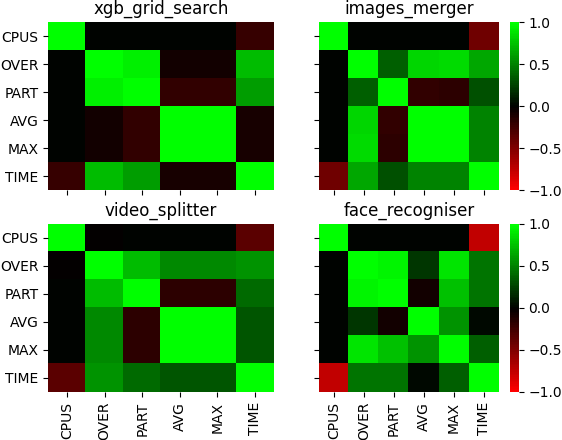
\includegraphics[width=1.0\textwidth]{corr}
	\end{minipage}
	\caption{Data columns pearson correlation per module.}
	\label{fig:corr}
\end{figure*}

To estimate time of a CAL module execution we create a machine learning model for each module. With each execution of the module within some application of the Baltic LSC system, we will get another data point to train our model. We will use the following features (explanatory variables)\footnote{As a docker container that will be used to execute a module do not use SWAP memory, RAM is not colerated with execution time. In this program we will not use modules with GPU support. Summarazing, the GPUs and RAM resources limits are not taken into account for modeling.} as an input data for a model:
\begin{enumerate}
	\item mCPUs limit - called \textit{mili cores} - the fraction of a physical CPU used to carry out the module execution,
	\item total size of an input data in bytes,
	\item max element size of an input data (if the input data is a set of files type it is the biggest part of data to be processed),
	\item average size of an input element,
	\item number of input data elements.
\end{enumerate}
This last three features make clear sense only if an input data is a set of files. Otherwise, if data is just a single file, the features can be a sort of data features representation carrying more detailed information about the data then only a total size. For the data frame the number of input elements can be eqaul to the number of columns. The max element size will be a quotient of the total size and the number of columns, and the average size will be equal to that quotient as well.

Obviously, our dependent value (that we are going to estimate) is an execution time of a module.

We create two CAL applications based on 4 modules with a different types of an input data. The first application, consisting of 3 modules, take the movie as an input data, marks faces of people on each frame and return the movie with marked people faces as an output data. The second one consist of just a single one module and it do a search of the best hyperparameters of XGBoost algorithm within parameters grid. Table~\ref{tab:modules} describe the modules that we used in the research.

\begin{table}[hbt!]
	\centering
	\caption{\label{tab:modules}Modules that we used in the research.}
	\begin{tabular}{|c c c|} 
		\hline
		ID (APP ID) & Name & Input data \\ [0.5ex] 
		\hline\hline
		1(1) & video\_splitter & video file \\ 
		\hline
		2(1) & face\_recogniser & image files \\
		\hline
		3(1) & images\_merger & image files \\
		\hline
		4(2) & xgb\_grid\_search & CSV file \\
		\hline
	\end{tabular}
\end{table}

For each module we created set of 10 different input data. Next, we ran the modules with the mentioned datas using different mCPUs resources (from 0.5 mCPUs up to 4.0 mCPUs with 0.5 step).

Finally, we received the data frame with the number of 4 (number of modules) * 8 (different mCPUs resources) * 10 (number of input data sets) = 320 rows that will be used to train and validate our models which part of is presented in the table~\ref{tab:example_df}.

\begin{table*}[!t]
	\centering
	\caption{\label{tab:example_df}Part of the data frame for models training and validation.}
	\begin{minipage}{0.9\linewidth}
		{\footnotesize
			\begin{tabular}{|c c c c c c >{\columncolor[gray]{0.9}}c|} 
				\hline
				Module ID & mCPUs & total size [B] & number of elements & max size [B] & average size [B] & time [s] \\ [0.5ex] 
				\hline\hline
				1 & 4.0 & 1703379 & 544 & 3131 & 3131 & 3.909 \\ 
				\hline
				1 & 4.0 & 809881 & 548 & 1477 & 1477 & 1.981  \\
				\hline
				1 & 4.0 & 1711796 & 1392 & 1229 & 1229 & 11.371 \\
				\hline
				... & ... & ... & ... & ... & ... & ... \\ [1ex] 
				\hline
			\end{tabular}
		}
	\end{minipage}
\end{table*}	